\documentclass[aspectratio=169]{beamer}

\usepackage[utf8]{inputenc}
\usetheme{Madrid}
\usecolortheme{beaver}
\usepackage{fontspec}
\usepackage{listings}

%Information to be included in the title page:
\title{fabric8}
\subtitle{An end-to-end development platform}
\author{Baiju Muthukadan}
\institute{Red Hat}
\date{@nogenerics}

\logo{
\includegraphics[height=1.5cm]{images/fabric8_icon.png}}

\begin{document}
\beamertemplatenavigationsymbolsempty

\setmainfont
[ Path = fonts/,
UprightFont = DejaVuSerif.ttf,
ItalicFont = DejaVuSerif-Italic.ttf,
BoldFont = DejaVuSerif-Bold.ttf,
BoldItalicFont = DejaVuSerif-BoldItalic.ttf,
Numbers={Lining, Monospaced},
] {DejaVu Serif}

\setsansfont
[ Path = fonts/,
UprightFont = DejaVuSans.ttf,
ItalicFont = DejaVuSans-Oblique.ttf,
BoldFont = DejaVuSans-Bold.ttf,
BoldItalicFont = DejaVuSans-BoldOblique.ttf,
Numbers={Lining, Monospaced},
] {DejaVu Sans}

\setmonofont
[ Path = fonts/,
UprightFont = DejaVuSansMono.ttf,
ItalicFont = DejaVuSansMono-Oblique.ttf,
BoldFont = DejaVuSansMono-Bold.ttf,
BoldItalicFont = DejaVuSansMono-BoldOblique.ttf,
Numbers={Lining, Monospaced},
] {DejaVu Sans Mono}


\newfontfamily{\vollkorn}
[ Path = fonts/,
UprightFont = Vollkorn-Regular.otf,
ItalicFont = Vollkorn-Italic.otf,
BoldFont = Vollkorn-Bold.otf,
BoldItalicFont = Vollkorn-BoldItalic.otf,
Numbers={Lining, Monospaced},
] {Vollkorn}

\newfontfamily{\dejavuserif}
[ Path = fonts/,
UprightFont = DejaVuSerif.ttf,
ItalicFont = DejaVuSerif-Italic.ttf,
BoldFont = DejaVuSerif-Bold.ttf,
BoldItalicFont = DejaVuSerif-BoldItalic.ttf,
Numbers={Lining, Monospaced},
] {DejaVu Serif}

\newfontfamily{\dejavusans}
[ Path = fonts/,
UprightFont = DejaVuSans.ttf,
ItalicFont = DejaVuSans-Oblique.ttf,
BoldFont = DejaVuSans-Bold.ttf,
BoldItalicFont = DejaVuSans-BoldOblique.ttf,
Numbers={Lining, Monospaced},
] {DejaVu Sans}

\newfontfamily{\dejavumono}
[ Path = fonts/,
UprightFont = DejaVuSansMono.ttf,
ItalicFont = DejaVuSansMono-Oblique.ttf,
BoldFont = DejaVuSansMono-Bold.ttf,
BoldItalicFont = DejaVuSansMono-BoldOblique.ttf,
Numbers={Lining, Monospaced},
] {DejaVu Sans Mono}

\frame{\titlepage}

\begin{frame}
  \frametitle{About Me}

  \begin{itemize}
  \item<1-> Senior Software Engineer, Red Hat
  \item<2-> FOSS Contributor (SMC, Koha, Zope, SaltStack, fabric8 etc.)
  \item<3-> Founded the Swathanthra Malayalam Computing (SMC) project in 2001 while studying at REC Calicut (NIT Kozhikode)
  \item<4-> Received the first Kenneth Gonsalves Award for contributions to the Python community in India
  \item<5-> Author of the book: A Comprehensive Guide to Go Programming \footnote{\url{https://golang.muthukadan.net}}
  \end{itemize}

\end{frame}

\begin{frame}
  \frametitle{Why fabric8?}

  \begin{itemize}
  \item<1-> \vollkorn{\Large "Now every company is a software company"}

  \item<2-> \vollkorn{\Large "Software is eating the world"}

  \item<3-> \vollkorn{\Large "You don’t have to be a software company to think like one"}

  \item<4-> \vollkorn{\Large "Every business will be a software business"}

  \end{itemize}


\end{frame}

\begin{frame}
  \frametitle{Why fabric8? ...}

  \begin{itemize}
  \item<1-> Microservices
  \item<2-> Containers (Docker/Moby, rkt)
  \item<3-> Container Orchestration (Kubernetes)
  \item<4-> PaaS (OpenShift)
  \end{itemize}

\end{frame}

\begin{frame}
  
\includegraphics[scale=.4]{images/fabric8_logo.png}
\end{frame}

\begin{frame}
  \frametitle{What fabric8 is solving?}

  \begin{itemize}

  \item<1-> An end-to-end development platform

  \item<2-> From ideation to beyond production

  \item<3-> Creation of cloud native applications and  microservices

  \item<4-> Plan, build, test and deploy your applications via pipelines

  \item<5-> Run and manage them with continuous improvement

  \end{itemize}

\end{frame}

\begin{frame}
  \frametitle{Schematic}
  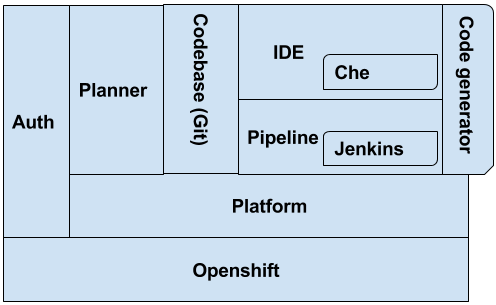
\includegraphics[scale=.65]{images/schematic.png}
\end{frame}

\begin{frame}
  \frametitle{Platform}

  \begin{itemize}
  \item<1-> Foundation
  \item<2-> RESTful API
  \item<3-> Backend in Go (Golang)
  \item<4-> Front-end in Angular 4/Patternfly
  \end{itemize}

\end{frame}

\begin{frame}
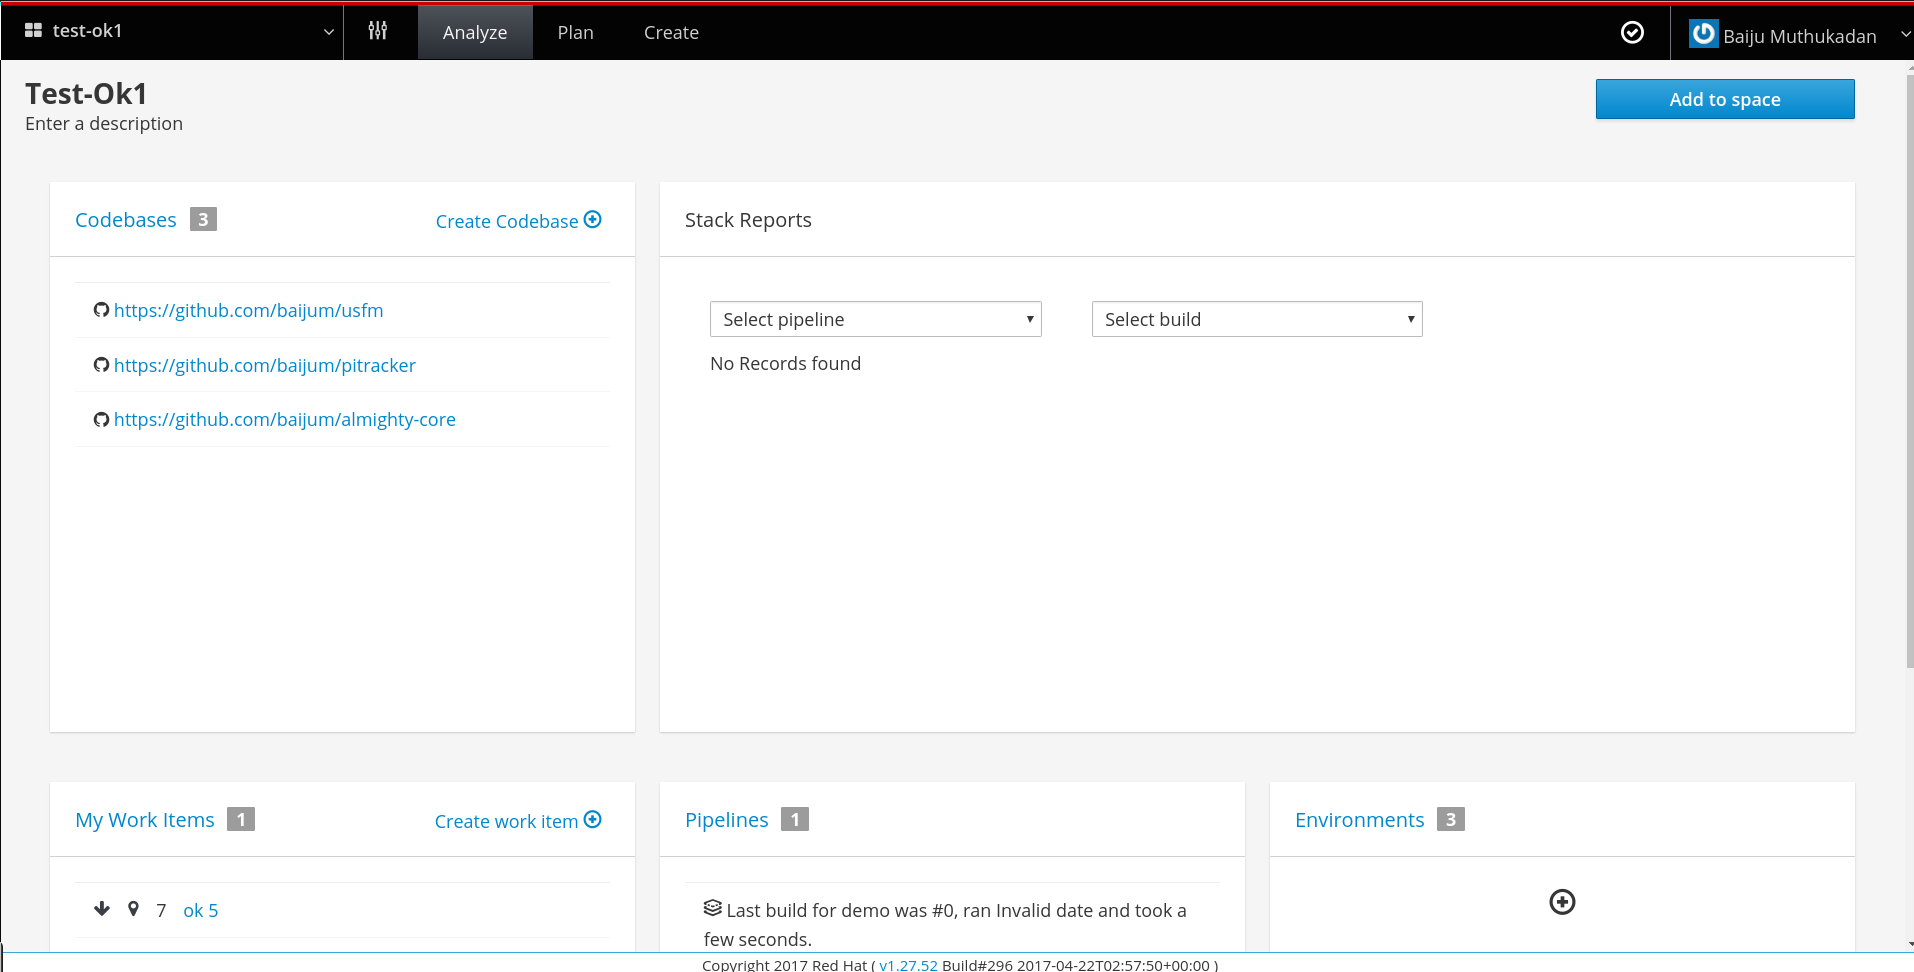
\includegraphics[scale=.27]{images/space.png}
\end{frame}

\begin{frame}
  \frametitle{Identity and Access Management}

  \begin{itemize}
  \item<1-> Built on Keycloak
  \item<2-> Single Sign On (OAuth, SAML)
  \item<3-> \url{http://www.keycloak.org}
  \end{itemize}

\end{frame}

\begin{frame}
  \frametitle{Planner}

  \begin{itemize}
  \item<1-> Project tracking
  \item<2-> Issue tracking
  \item<3-> RESTful API
  \item<4-> Backend in Go (Golang)
  \item<5-> Front-end in Angular 4/Patternfly
  \end{itemize}

\end{frame}

\begin{frame}
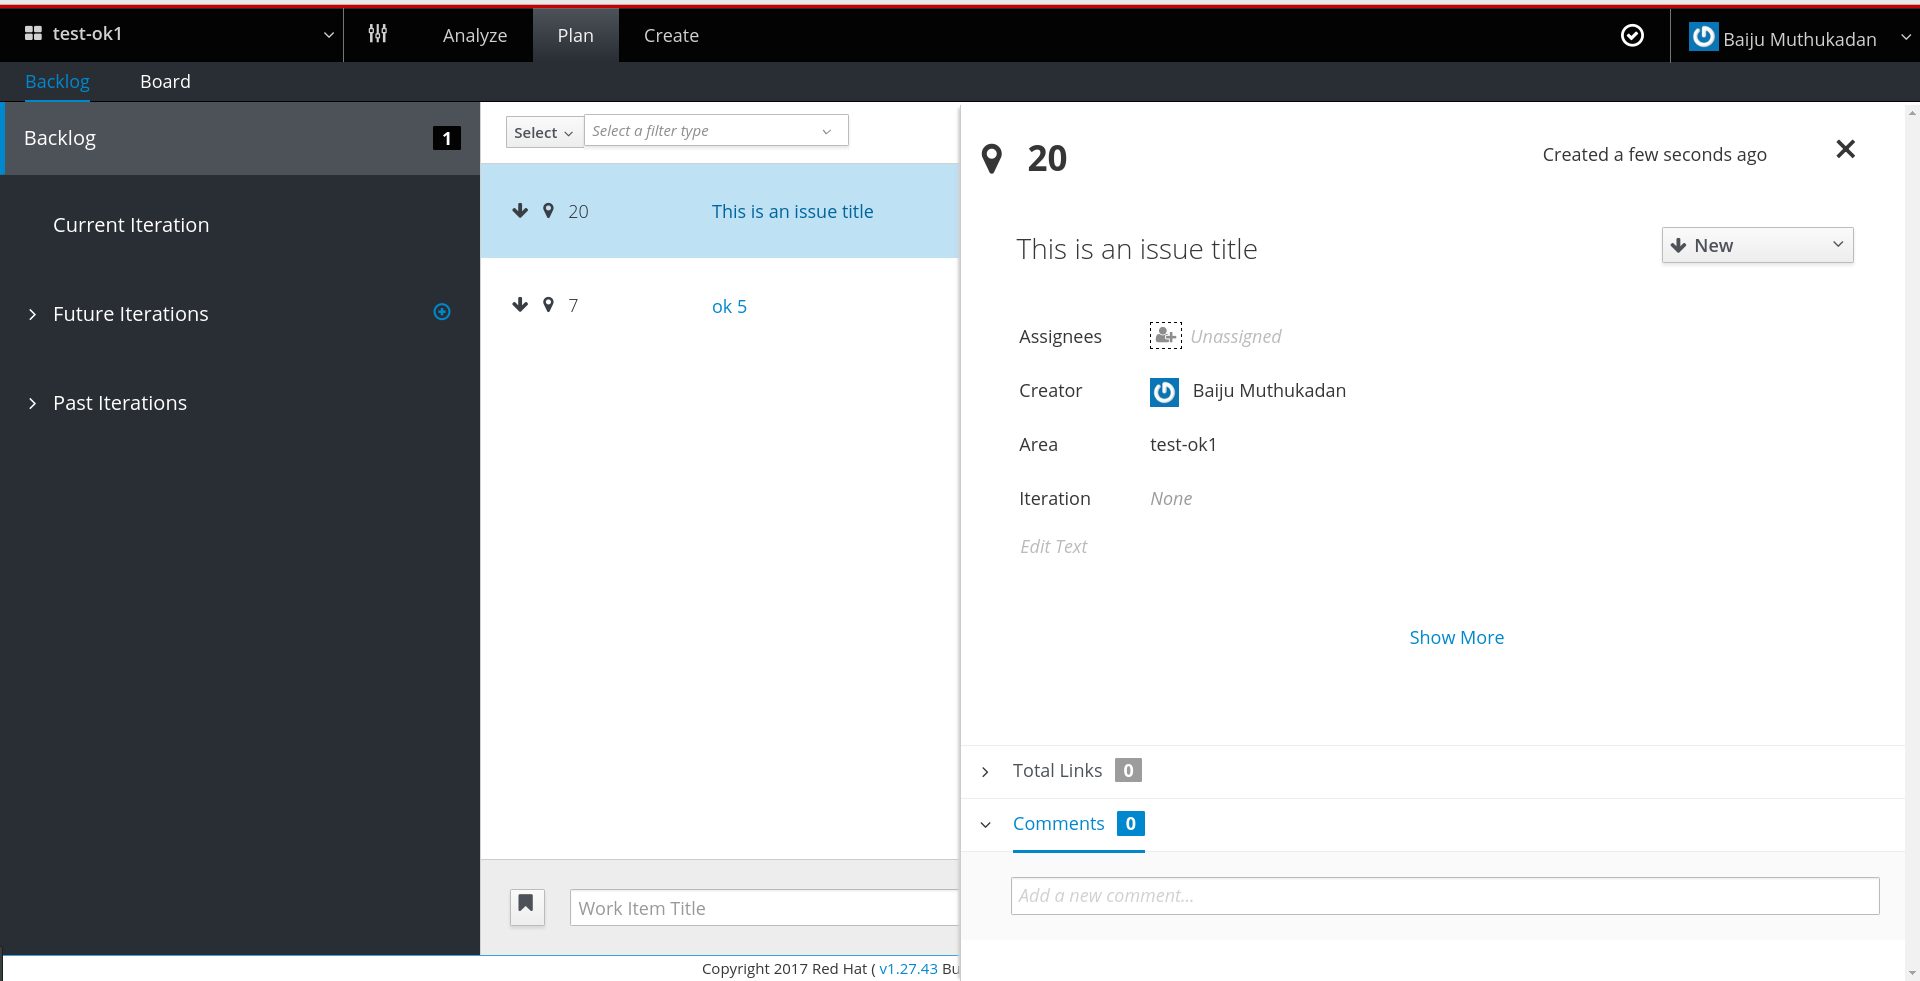
\includegraphics[scale=.2]{images/planner.png}
\end{frame}

\begin{frame}
  \frametitle{Code Editor}

  \begin{itemize}
  \item<1-> Built on Eclipse Che
  \item<2-> \url{http://www.eclipse.org/che}
  \end{itemize}

\end{frame}

\begin{frame}
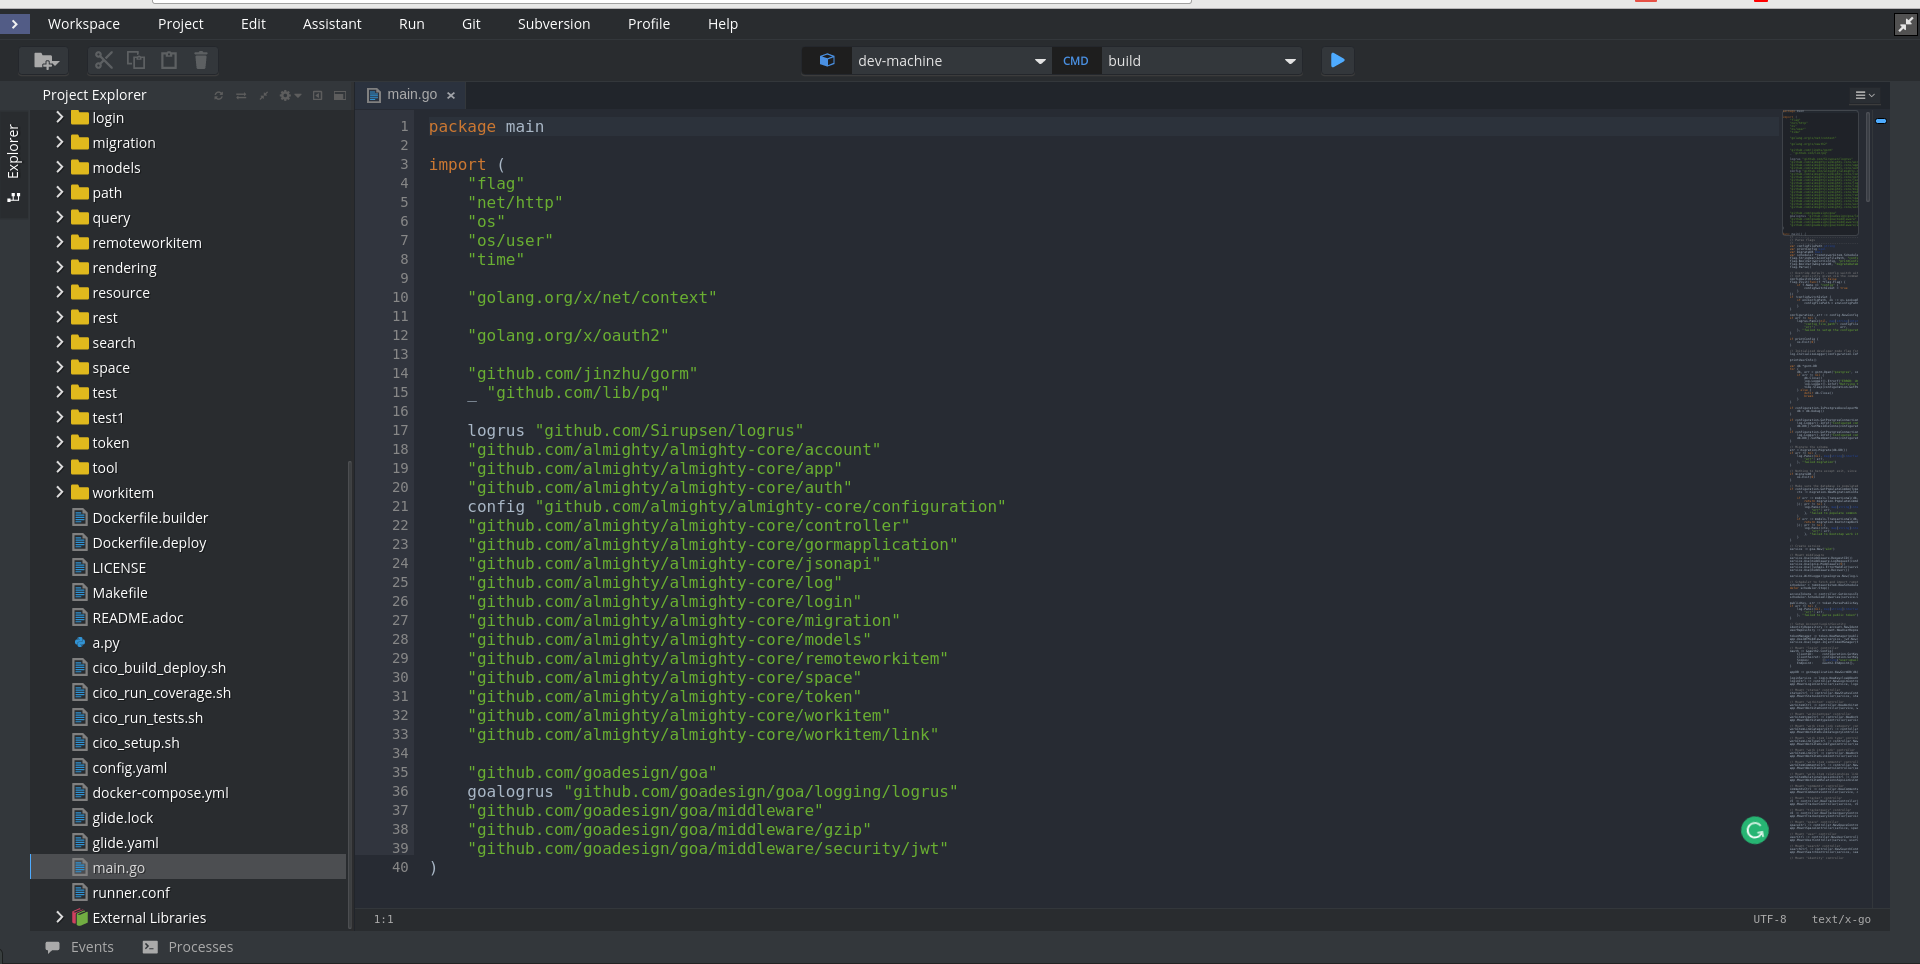
\includegraphics[scale=.2]{images/che.png}
\end{frame}

\begin{frame}
  \frametitle{Pipeline}

  \begin{itemize}
  \item<1-> Built on Jenkins
  \item<2-> https://jenkins.io
  \end{itemize}

\end{frame}

\begin{frame}
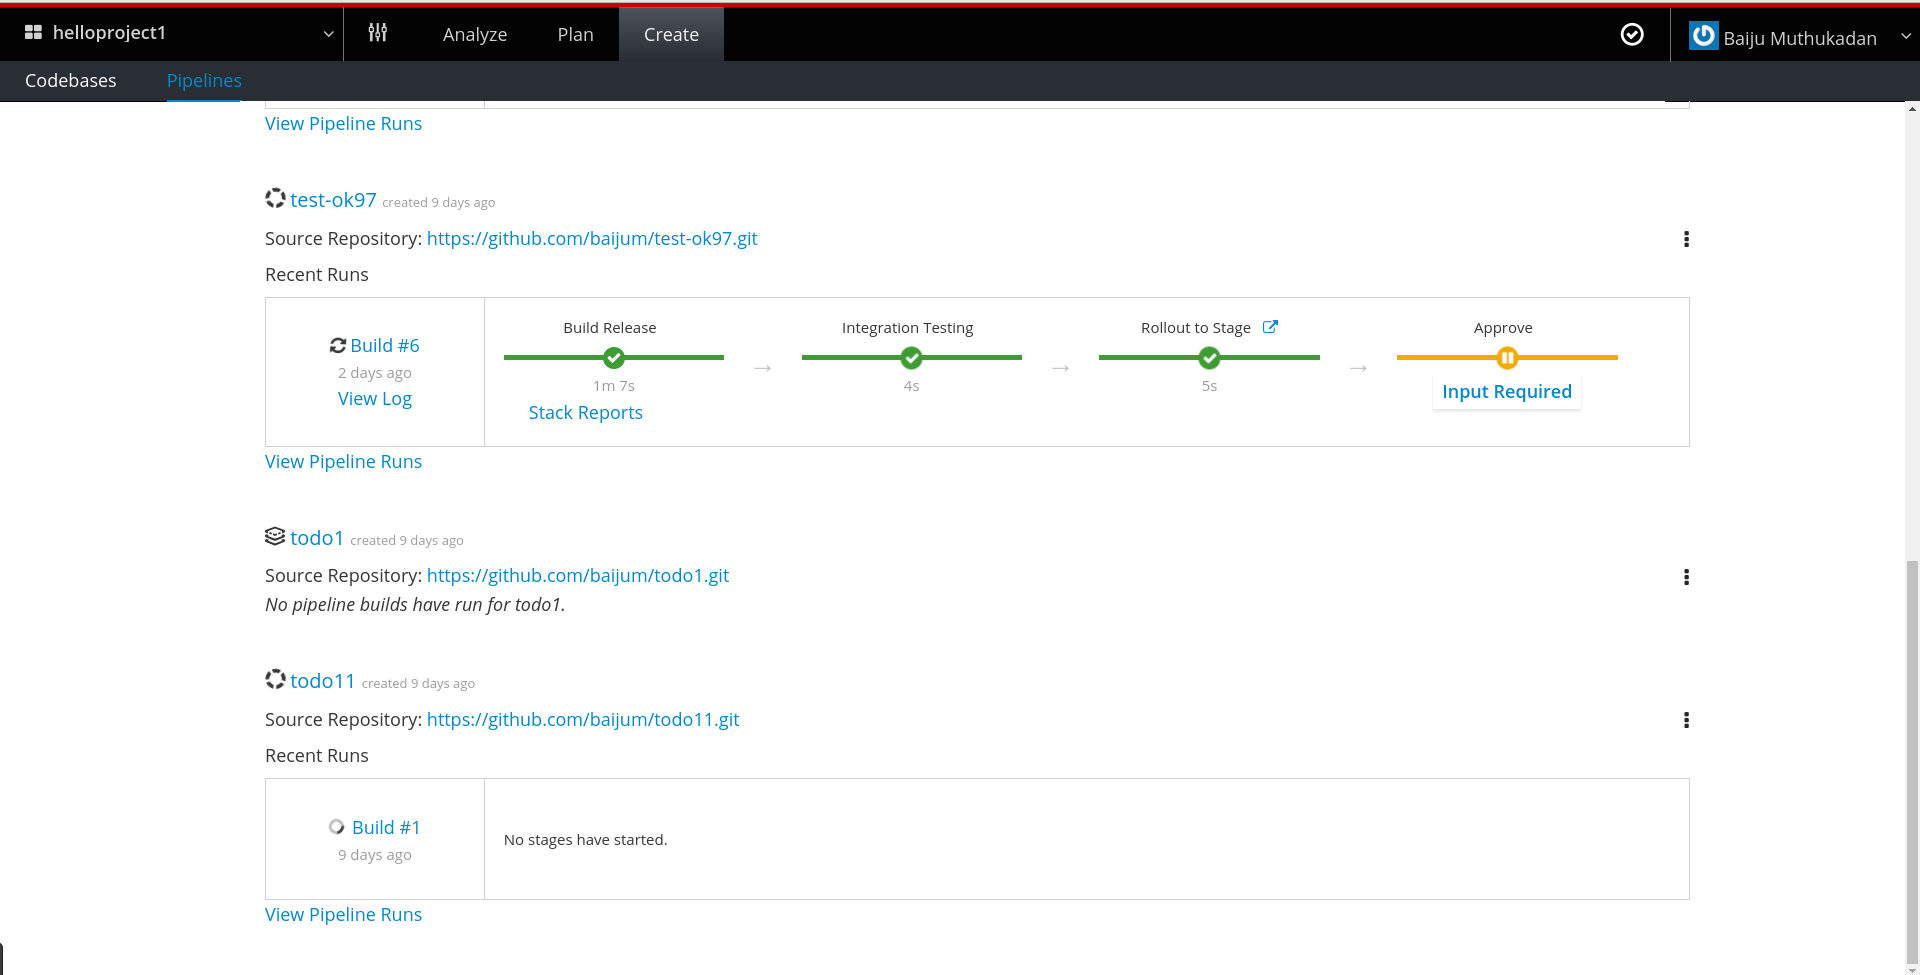
\includegraphics[scale=.27]{images/pipeline.png}
\end{frame}

\begin{frame}
  \frametitle{Deployment}

\begin{itemize}
  \item<1-> OpenShift
  \item<2-> \url{https://www.openshift.org}
\end{itemize}
\end{frame}



\begin{frame}
  \frametitle{Demo}

  (Video demo - 4 minutes)

\end{frame}


\begin{frame}
  \frametitle{Conclusion}

\begin{itemize}
  \item<1-> Streamlining software development from ideation to production
  \item<2-> Contributions are welcome!
  \item<3-> \url{https://fabric8.io}
  \item<3-> \url{https://github.com/fabric8io}
\end{itemize}
\end{frame}


\begin{frame}%%     1
\begin{center}
{\huge Thank You!}\\[1cm]
{\large \href{https://twitter.com/nogenerics}{@nogenerics}}
\end{center}
\end{frame}


\end{document}
